\documentclass[10pt]{beamer}

\usepackage[utf8]{inputenc}
\usepackage{hyperref}
\hypersetup{colorlinks=true,linkbordercolor=blue,linkcolor=white,urlcolor=blue,pdfborderstyle={/S/U/W 1}}

\usepackage[scaled]{helvet}
\usepackage[T1]{fontenc}
\usetheme{Berkeley}
\beamertemplatenavigationsymbolsempty
\setbeamertemplate{headline}{}

\setbeamersize{sidebar width left=1.5cm}
\setbeamerfont{section in sidebar}{size=\fontsize{6}{6}\selectfont}
\setbeamerfont{title in sidebar}{size=\fontsize{6}{6}\selectfont}

\title{Geocoding mit Photon in FoodChain-Lab}
\date{}
 
\begin{document}
\maketitle

\section{Topics}
\begin{frame}
\leftskip1em\textbf{Lernen Sie}
	\begin{itemize}
    \item was Geocoding ist
    \item wie der Geocoding-Service (Photon) verwendet wird
	\end{itemize}
\end{frame}
 
\section{1}
\begin{frame}
	\begin{center}
  		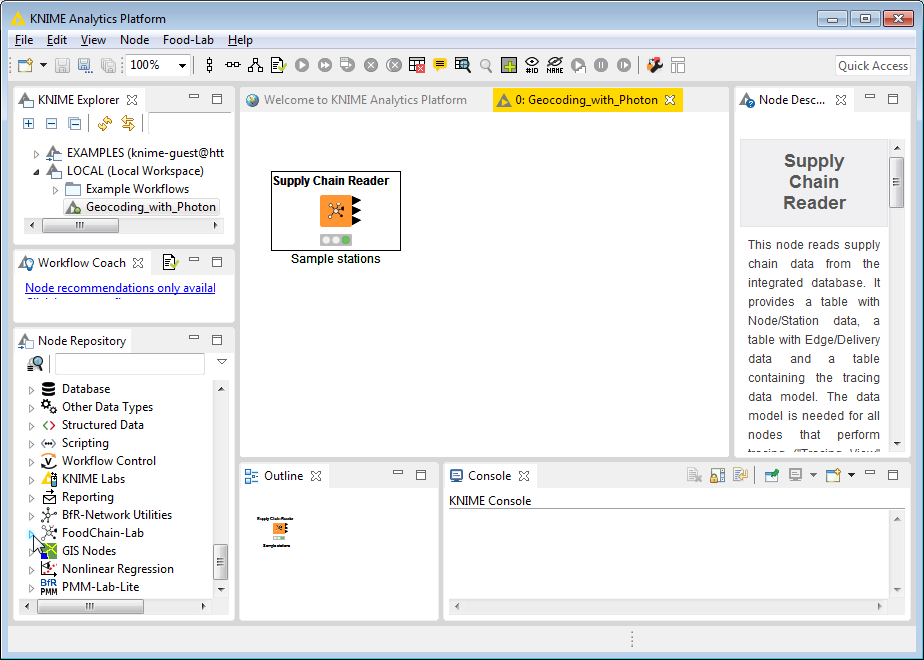
\includegraphics[height=0.6\textheight]{1.png}
	\end{center}
	\begin{itemize}
		\item Importieren Sie den Geocoding Workflow von  \textcolor{blue}{\underline{\href{https://github.com/SiLeBAT/BfROpenLabResources/raw/master/GitHubPages/workflows/Geocoding\_with\_Photon.knwf}{``Geocoding\_with\_Photon.knwf''}}}.
	\end{itemize}
\end{frame}

\section{2}
\begin{frame}
	\begin{center}
  		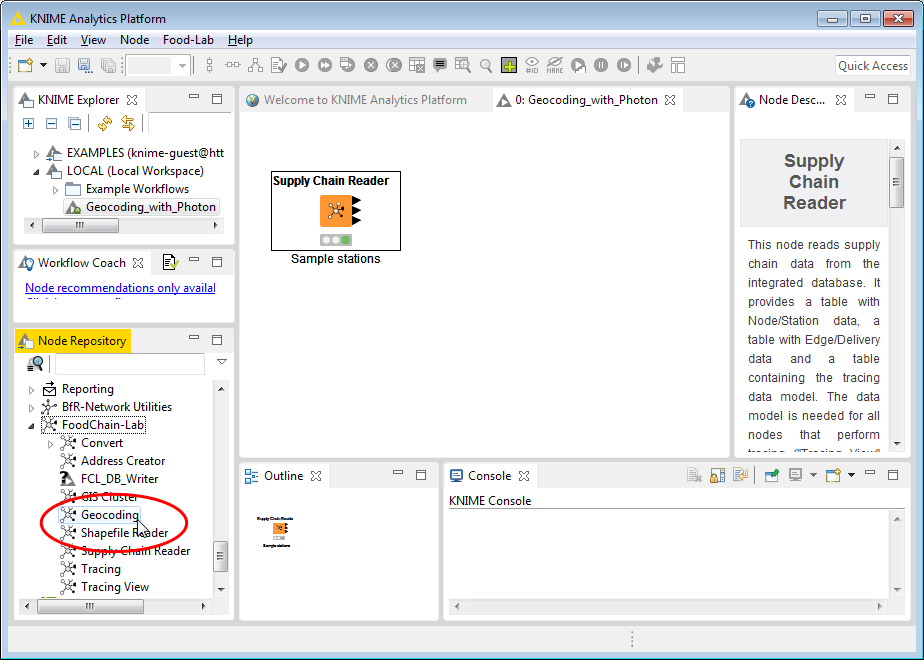
\includegraphics[height=0.6\textheight]{2.png}
	\end{center}
	\begin{itemize}
        \item Um den Geocoding Service zu nutzen muss der \textbf{Geocoding} Knoten hinzugefügt werden. 
        \item Falls der \textbf{Supply Chain Reader} ausgewählt ist, kann der Knoten durch einen Doppelklick auf den  \textbf{Geocoding} Knoten im \textbf{Node Repository} hinzugefügt werden. 
	\end{itemize}
\end{frame}

\section{3}
\begin{frame}
	\begin{center}
  		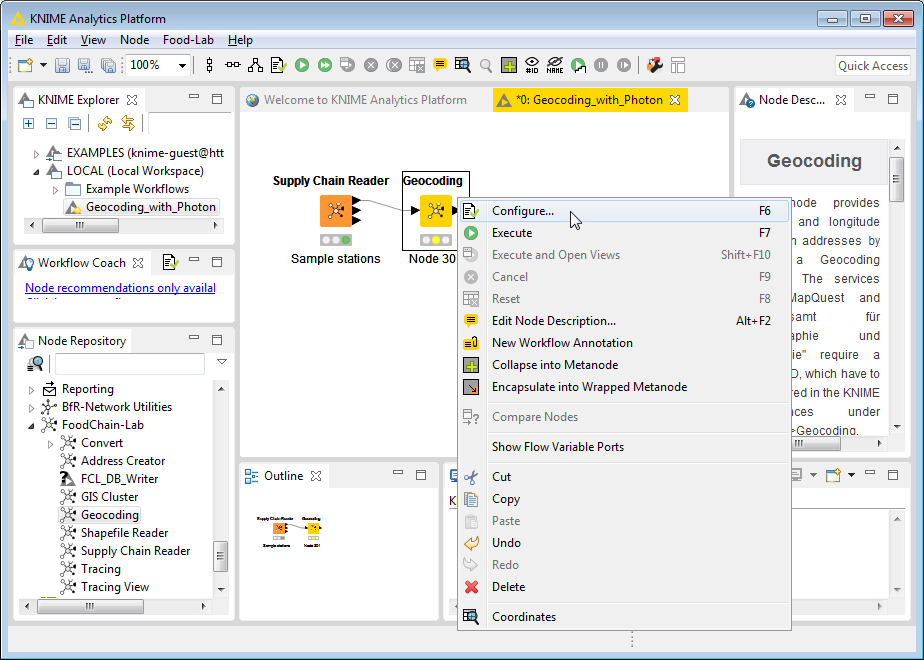
\includegraphics[height=0.6\textheight]{3.png}
	\end{center}
	\begin{itemize}
        \item Ein \textbf{Geocoding} Knoten wurde zum Workflow hinzugefügt. Er ist verbunden mit dem \textbf{SupplyChainReader} und muss konfiguriert werden.
		%\item The \textbf{Geocoding} node has to be set up (to use Photon)
		\item Öffnen Sie den Konfigurationsdialog durch einen Doppelklick auf den Knoten oder durch Benutzung des Kontextmenüs (Rechtsklick auf den Knoten).
		%\item In this tutorial we are using the Photon Geocoding service.
	\end{itemize}
\end{frame}

\section{4}
\begin{frame}
	\begin{center}
  		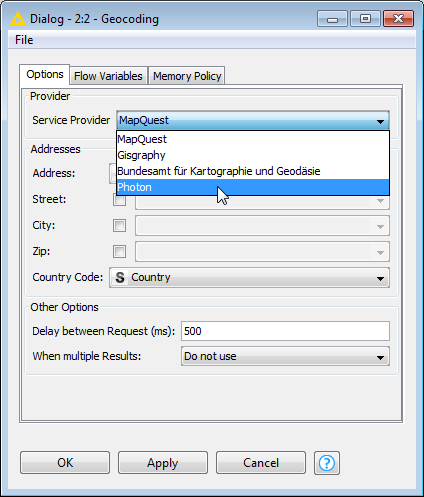
\includegraphics[height=0.6\textheight]{4.png}
	\end{center}
	\begin{itemize}
        \item Setzen Sie den \textbf{Service Provider} auf \textbf{Photon}.
		%\item The Geocoding-Node has to be configured (to use Photon)
		%\item Open its configuration by double clicking on it or by using its context menue (right click on the node)
		%\item In this tutorial we are using the Photon Geocoding service.
	\end{itemize}
\end{frame}

\section{5}
\begin{frame}
	\begin{center}
  		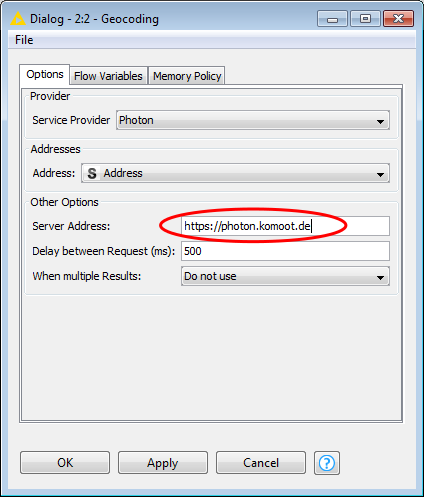
\includegraphics[height=0.6\textheight]{5.png}
	\end{center}
	\begin{itemize}
        \item Die \textbf{Address} ist passend gesetzt.
		\item Sie müssen die \textbf{Server Address} eingeben. Dafür können Sie \textbf{https://photon.komoot.de} nutzen, einen öffentlich verfügbaren Dienst. 
		%\item The Geocoding-Node has to be configured (to use Photon)
		%\item Open its configuration by double clicking on it or by using its context menue (right click on the node)
		%\item In this tutorial we are using the Photon Geocoding service.
	\end{itemize}
\end{frame}

\section{6}
\begin{frame}
	\begin{center}
  		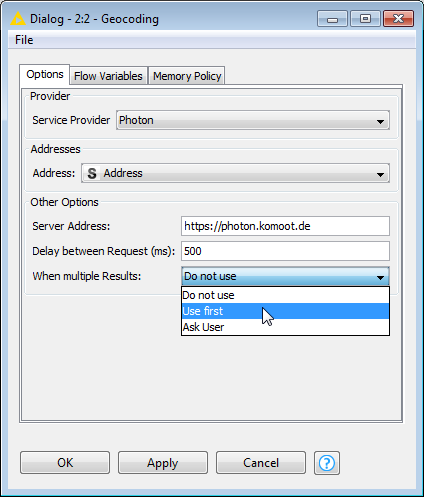
\includegraphics[height=0.5\textheight]{6.png}
	\end{center}
	\begin{itemize}
		\item Es passiert häufig, dass der Geocoding Service zu einer Anfrage mehrere Resultate liefert (z.B. wenn es mehrere Straßen mit demselben Name in einer Stadt gibt).
		\item Wir müssen definieren was in diesem Fall passieren soll: kein Resultat nehmen, das erste Resultat nehmen oder das passende Resultat manuell auswählen.
		\item Manuelles Auswählen ist bei großen Datenmengen sehr arbeitsaufwendig, deshalb wählen wir hier einfach \textbf{Use first} und klicken \textbf{OK}.
	\end{itemize}
\end{frame}

\section{7}
\begin{frame}
	\begin{center}
  		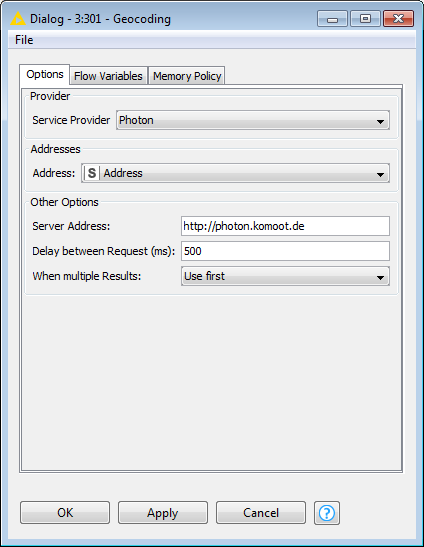
\includegraphics[height=0.5\textheight]{7.png}
	\end{center}
	\begin{itemize}
    \item In diesem tutorial wählen Sie bitte ``Use first'' und klicken ``OK''.
	\end{itemize}
\end{frame}

\section{8}
\begin{frame}
	\begin{center}
  		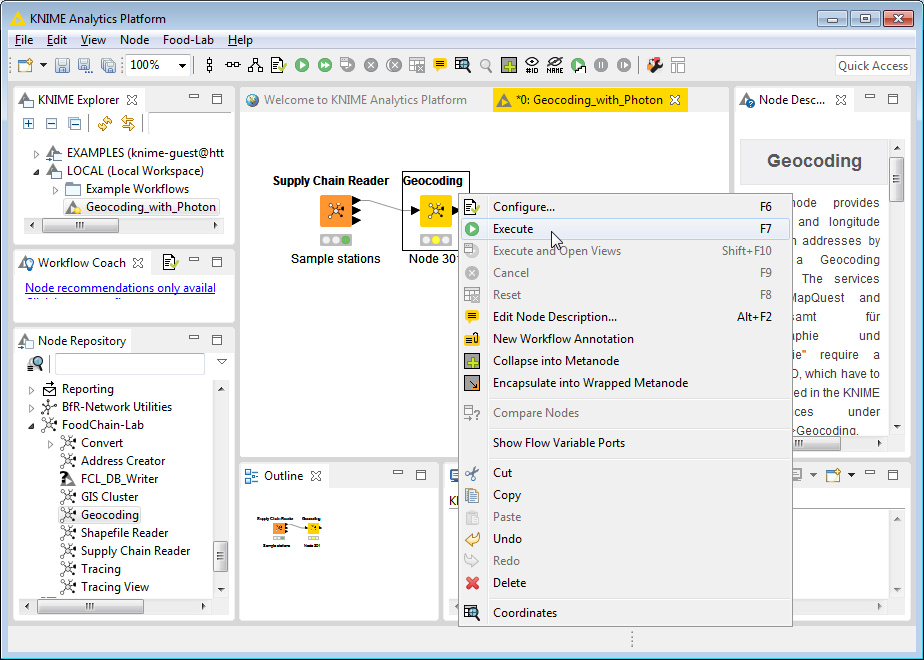
\includegraphics[height=0.6\textheight]{8.png}
	\end{center}
	\begin{itemize}
		\item Machen Sie einen Rechtsklick auf den \textbf{Geocoding}-Knoten und wählen Sie \textbf{Execute}.
	\end{itemize}
\end{frame}

\section{9}
\begin{frame}
	\begin{center}
  		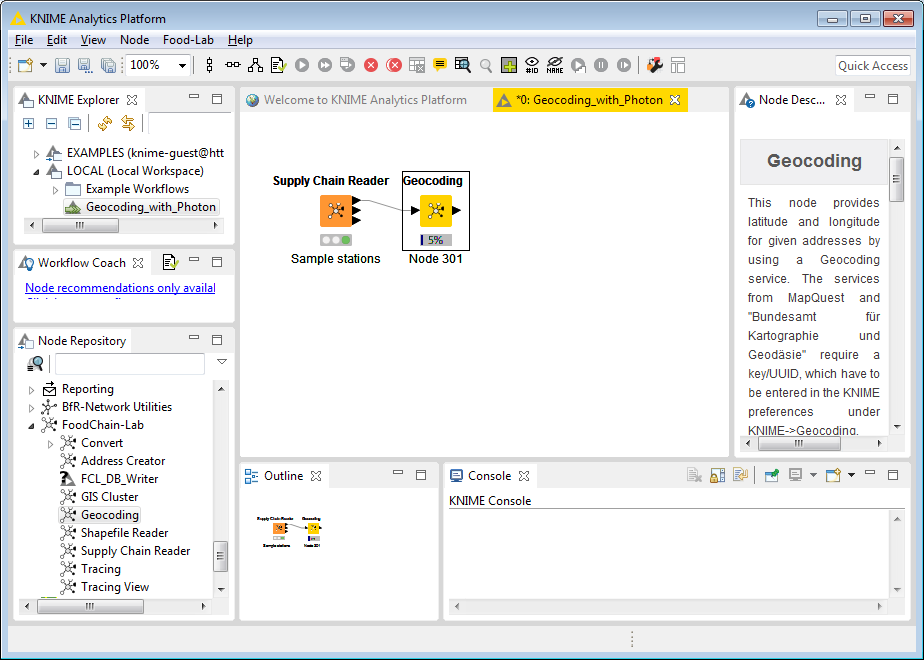
\includegraphics[height=0.6\textheight]{9.png}
	\end{center}
	\begin{itemize}
		\item Die Ausführung kann eine Weile dauern.
		\item Unter dem Knoten wird angezeigt welcher Prozentsatz der Daten bereits bearbeitet wurde.
	\end{itemize}
\end{frame}

\section{10}
\begin{frame}
	\begin{center}
  		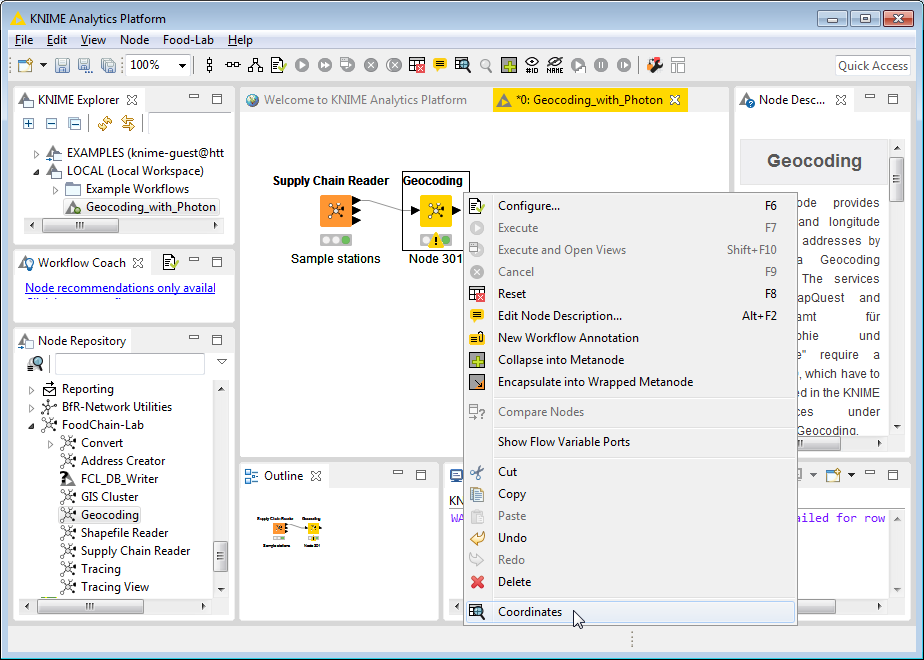
\includegraphics[height=0.6\textheight]{10.png}
	\end{center}
	\begin{itemize}
		\item Wenn die Ausführung beendet ist, können wir uns die Resultate anschauen.
		\item Machen Sie einen Rechtsklick auf den \textbf{Geocoding}-Knoten und wählen Sie \textbf{Coordinates}.
	\end{itemize}
\end{frame}

\section{11}
\begin{frame}
	\begin{center}
  		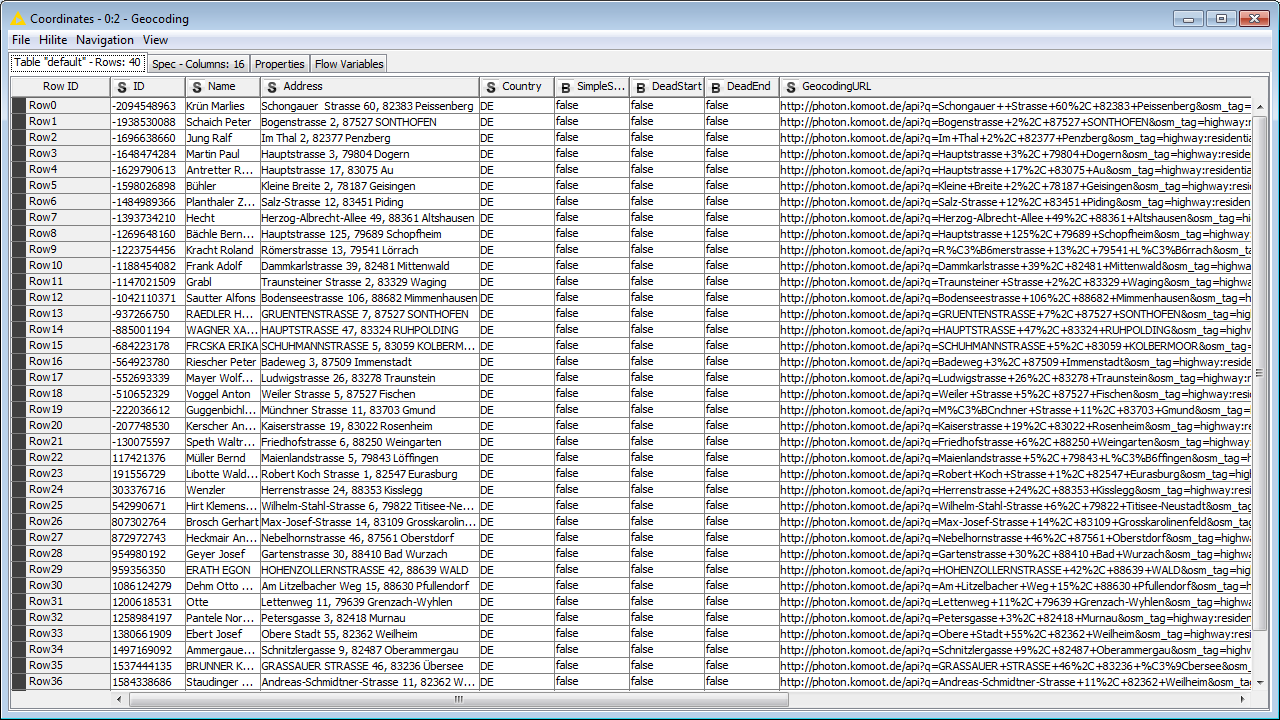
\includegraphics[height=0.6\textheight]{11.png}
	\end{center}
	\begin{itemize}
		\item In dem Dialog können Sie sich die gesamte Datentabelle anschauen.
	\end{itemize}
\end{frame}

\section{12}
\begin{frame}
	\begin{center}
  		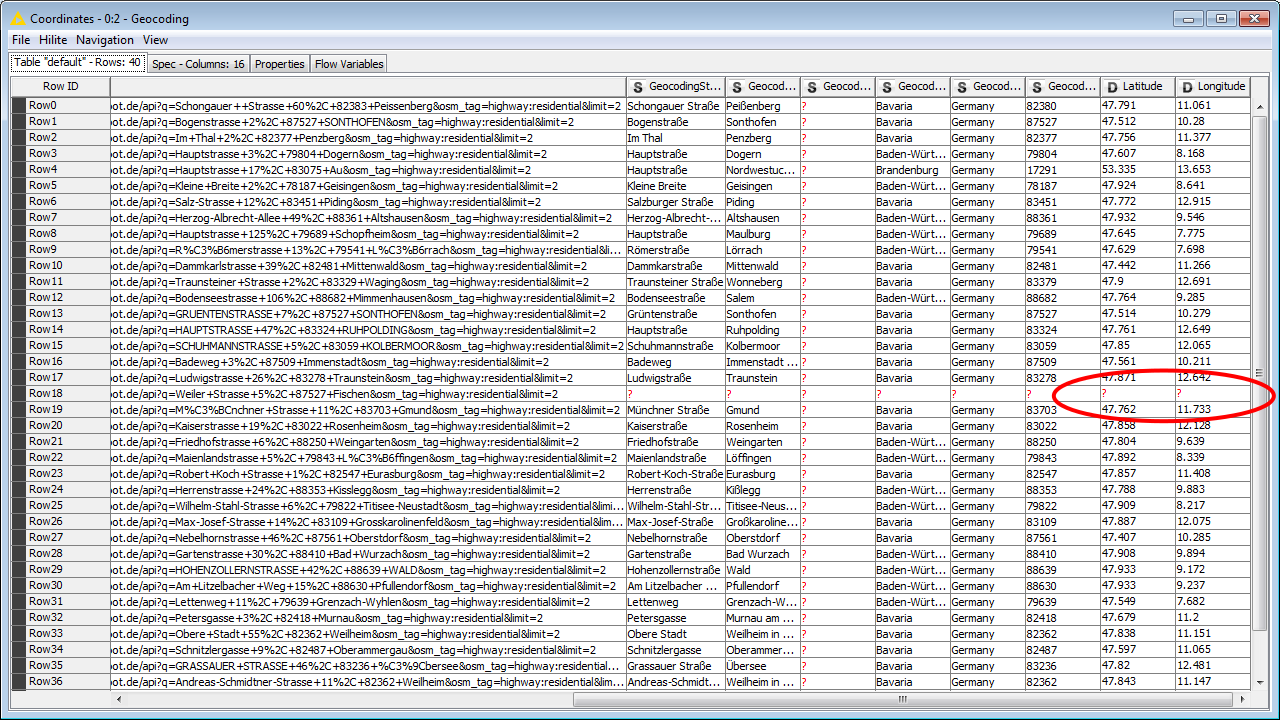
\includegraphics[height=0.6\textheight]{12.png}
	\end{center}
	\begin{itemize}
		\item Scrollen Sie ganz nach rechts um sich die Spalten mit geographischer Breite und Länge anzuschauen (die zwei Spalten ganz rechts).
		\item Für 39 von 40 Addressen konnten die Breiten und Längen gefunden werden. Eine Geocoding Anfrage lieferte keine Ergebnisse. 
	\end{itemize}
\end{frame}

\end{document}
